% Mana Maths Notes template
\documentclass[aspectratio=169,12pt]{beamer}
\usepackage{amsmath}
\usepackage{amssymb}
\usepackage{array}
\usepackage[most]{tcolorbox}
\usepackage{graphicx}
\usepackage{tikz}
\usepackage[sfdefault,lf]{FiraSans}
\renewcommand{\familydefault}{\sfdefault}
\setlength{\parindent}{0pt}
\everymath{\displaystyle}

\setbeamertemplate{navigation symbols}{}
\setbeamertemplate{footline}{}
\setbeamertemplate{headline}{}
\setbeamertemplate{blocks}[rounded][shadow=false]

\definecolor{mmtanPage}{HTML}{F3E8D7}
\definecolor{mmtanSoft}{HTML}{F8F0E5}
\definecolor{mmgreenDeep}{HTML}{244B2C}
\definecolor{mmgreenLeaf}{HTML}{5D8A56}
\definecolor{mmgreenSoft}{HTML}{E4EFD9}
\definecolor{mmtext}{HTML}{163221}
\definecolor{mmwarn}{HTML}{8F2F36}
\definecolor{mmwarnSoft}{HTML}{F8E8EA}

\setbeamercolor{background canvas}{bg=mmtanPage}
\setbeamercolor{normal text}{fg=mmtext,bg=mmtanPage}
\setbeamercolor{block title}{fg=mmgreenDeep,bg=mmgreenSoft}
\setbeamercolor{block body}{fg=mmtext,bg=mmtanSoft}
\setbeamercolor{block title example}{fg=mmgreenDeep,bg=mmgreenSoft}
\setbeamercolor{block body example}{fg=mmtext,bg=white}
\setbeamercolor{block title alerted}{fg=mmwarn,bg=mmwarnSoft}
\setbeamercolor{block body alerted}{fg=mmtext,bg=white}

\newtcolorbox{MMCard}[2][]{enhanced,breakable=false,colback=#2,colframe=black,boxrule=1.5pt,arc=8pt,left=6pt,right=6pt,top=5pt,bottom=5pt,before skip=0pt,after skip=0pt,#1}
\newcommand{\KoruIcon}{\raisebox{-0.2em}{\includegraphics[height=1.05em]{../../../manamaths/SITE/header-logo.png}}}
\newcommand{\NotesTitle}[1]{{\colorbox{mmtanSoft}{\parbox{0.975\linewidth}{\vspace{0.20em}\hspace{0.25em}{\LARGE\bfseries\textcolor{mmgreenDeep}{#1}\hfill\KoruIcon}\vspace{0.20em}}}\par\vspace{0.26em}{\color{mmgreenLeaf}\rule{\linewidth}{2.2pt}}\par\vspace{0.20em}}}
\newcommand{\SectionTitle}[1]{{\large\bfseries\textcolor{mmgreenDeep}{#1}}\par\vspace{0.06em}}
\newcommand{\GreenDivider}{\par\vspace{0.02em}{\color{mmgreenLeaf}\rule{\linewidth}{3.0pt}}\par\vspace{0.05em}}
\newcommand{\KeyIdea}[1]{\begin{MMCard}[title={\textbf{Key idea}},colbacktitle=mmgreenSoft,coltitle=mmgreenDeep]{mmtanSoft}\small #1\end{MMCard}}
\newcommand{\WorkedExample}[2]{\begin{MMCard}[title={\textbf{#1}},colbacktitle=mmgreenSoft,coltitle=mmgreenDeep]{white}\small #2\end{MMCard}}
\newcommand{\CommonMistake}[1]{\begin{MMCard}[title={\textbf{Common mistake}},colbacktitle=mmwarnSoft,coltitle=mmwarn]{white}\small #1\end{MMCard}}
\newcommand{\TryThese}[1]{\begin{MMCard}[title={\textbf{Try these}},colbacktitle=mmgreenSoft,coltitle=mmgreenDeep]{mmtanSoft}\small #1\end{MMCard}}
\newcommand{\StepLine}[2]{\textbf{#1.} #2\par\vspace{0.05em}}

\begin{document}

% Slide 1: What gradient means for curves
\begin{frame}[t]\NotesTitle{Gradient of Tangents on Curves}
\begin{columns}[T,onlytextwidth]
\begin{column}{0.48\textwidth}
\KeyIdea{The \textbf{gradient} of a curve at a point is the gradient of the \textbf{tangent line}. Unlike straight lines, curves have a different gradient at every point.}

\vspace{0.1em}
\SectionTitle{How to estimate gradient}
\small
$\bullet$ Draw the tangent line at the point.\\
$\bullet$ Pick two grid intersection points on the tangent.\\
$\bullet$ $m = \frac{\Delta y}{\Delta x}$ (rise over run).\\
$\bullet$ Horizontal tangent $\Rightarrow$ $m=0$ (turning point).
\end{column}
\begin{column}{0.48\textwidth}
\WorkedExample{Estimating gradient from a tangent}{
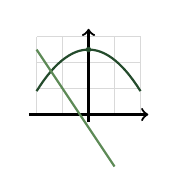
\begin{tikzpicture}[scale=0.33,baseline=(current bounding box.center)]
\draw[thin,gray!30] (-2,0) grid (2,3);
\draw[thick,->] (-2.3,0) -- (2.3,0);
\draw[thick,->] (0,-0.3) -- (0,3.3);
\draw[thick,mmgreenDeep,samples=30,domain=-2:2] plot(\x,{-0.4*(\x-0)*(\x-0)+2.5});
\draw[thick,mmgreenLeaf] (-2,2.5) -- (1,-2);
\fill[mmgreenDeep] (0,2.5) circle (3pt);
\end{tikzpicture}\\[1mm]
Rise $=-4$, Run $=1 \Rightarrow m=-4$
}
\end{column}
\end{columns}
\end{frame}

% Slide 2: Gradient signs and turning points
\begin{frame}[t]\NotesTitle{Gradient of Tangents on Curves}
\begin{columns}[T,onlytextwidth]
\begin{column}{0.48\textwidth}
\SectionTitle{Gradient signs}
\centering
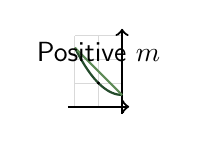
\begin{tikzpicture}[scale=0.30]
\draw[thin,gray!30] (-2,0) grid (0,3);
\draw[thick,->] (-2.3,0) -- (0.3,0);
\draw[thick,->] (0,-0.3) -- (0,3.3);
\draw[thick,mmgreenDeep,samples=20,domain=-2:0] plot(\x,{0.5*\x*\x+0.5});
\draw[thick,mmgreenLeaf] (-2,2.5) -- (0,0.5);
\fill (-1,1) circle (2pt);
\node[above] at (-1,1.5){Positive $m$};
\end{tikzpicture}
\hspace{0.3cm}
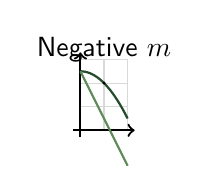
\begin{tikzpicture}[scale=0.30]
\draw[thin,gray!30] (0,0) grid (2,3);
\draw[thick,->] (-0.3,0) -- (2.3,0);
\draw[thick,->] (0,-0.3) -- (0,3.3);
\draw[thick,mmgreenDeep,samples=20,domain=0:2] plot(\x,{-0.5*\x*\x+2.5});
\draw[thick,mmgreenLeaf] (0,2.5) -- (2,-1.5);
\fill (1,2) circle (2pt);
\node[above] at (1,2.5){Negative $m$};
\end{tikzpicture}

\vspace{0.1em}
\KeyIdea{A \textbf{positive gradient} ($m>0$) means the curve slopes upward. \textbf{Negative} ($m<0$) means it slopes downward. At a \textbf{turning point}, $m=0$ (horizontal tangent).}
\end{column}
\begin{column}{0.48\textwidth}
\SectionTitle{Increasing / Decreasing}
If $m>0$, function is \textbf{increasing}.
If $m<0$, function is \textbf{decreasing}.
If $m=0$, \textbf{stationary} (turning point).

\vspace{0.2em}
\WorkedExample{Identifying turning points}{
\centering
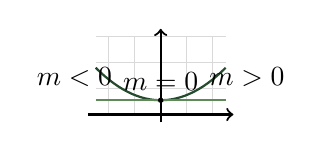
\begin{tikzpicture}[scale=0.33,baseline=(current bounding box.center)]
\draw[thin,gray!30] (-2.5,0) grid (2.5,3);
\draw[thick,->] (-2.8,0) -- (2.8,0);
\draw[thick,->] (0,-0.3) -- (0,3.3);
\draw[thick,mmgreenDeep,samples=30,domain=-2.5:2.5] plot(\x,{0.2*(\x-1.5)*(\x+1.5)+1});
\draw[thick,mmgreenLeaf] (-2.5,0.55) -- (2.5,0.55);
\fill (0,0.55) circle (3pt);
\node[above] at (0,0.55){$m=0$};
\node[right] at (1.5,1.45){$m>0$};
\node[left] at (-1.5,1.45){$m<0$};
\end{tikzpicture}\\
Gradient changes $-\to0\to+$ = \textbf{minimum}.
}
\end{column}
\end{columns}
\end{frame}

% Slide 3: Stationary point types
\begin{frame}[t]\NotesTitle{Gradient of Tangents on Curves}
\SectionTitle{Stationary point types}
\begin{columns}[T,onlytextwidth]
\begin{column}{0.48\textwidth}
\textbf{Maximum}: gradient $+\to0\to-$ (curve peaks)\\[1mm]
\textbf{Minimum}: gradient $-\to0\to+$ (curve troughs)\\[1mm]
\textbf{Inflection}: gradient $0$ but sign unchanged (curve flattens briefly then continues)
\end{column}
\begin{column}{0.48\textwidth}
\TryThese{
1. A tangent slopes up 2 for 1 right. What is $m$?\\[1mm]
2. Gradient is $+$ then $0$ then $-$. Max or min?\\[1mm]
3. At a turning point, what is the gradient?}
\vspace{0.2em}
\small \textbf{Answers:} 1. $m=2$ \quad 2. Max \quad 3. $m=0$
\end{column}
\end{columns}
\end{frame}

\end{document}
